\label{sec:results}

As a preliminary benchmark, we begin by determining the maximum
obtainable throughput through message passing available in both
\texttt{Distributed.jl} and \texttt{ArrayChannels.jl}, compared to an
OpenMPI 4.0.0 baseline\footnote{Ping-pong implementations for evaluation
  are available in the project repository:
  https://github.com/rohanmclure/ArrayChannels.jl/tree/master/example.
  Reference implementations for MPI are obtained from
  https://github.com/ParRes/Kernels/tree/master/MPI1, and built with
  default parameters but with \texttt{-O3} enabled.}. Afterwards we
assess the performance of the \texttt{ArrayChannels.jl} communication
model on the data parallelism benchmarks contained in the Intel PRK. The
Intel PRK implementations accomodate arbitrary numbers of cores, and we
obtain results for core counts ranging between one and fourteen.

Results were obtained on a single compute node with two 8-core Intel
Xeon Gold 6134 (@ 3.20GHz) sockets\footnote{Results were obtained on
  Ubuntu 18.04.2 LTS and Julia version 1.1.0. The MPI implemenations
  were compiled under \texttt{gcc} version 4.7.0 with OpenMPI 4.0.0.}.
Each CPU featured dual-lane Hyper-Threading and 24.75MB of last-level
cache. We took the average performance reading after evaluating the
benchmarks a number of times for each problem size / core count. During
evaluation, each kernel is executed under 1000 iterations with an
additional warm-up iteration. This reduces the impact of runtime events
such as \emph{JIT} compilation on performance readings to indicate
eventual performance outcomes \cite{blackburn, kulkarni}.

\subsection{Ping-Pong}
\label{sec:pingpong-results}

In figure~\ref{fig:pingpong-results}, we provide a profile of the
maximum obtainable throughput that can be achieved for messages of a
certain size. The MPI and \texttt{Distributed.jl} implementations
feature a steep drop-off in throughput for messages greater than 8MB in
size, suggesting that the maximum communication bandwidth has been
obtained. For larger message sizes, both implementations yield
deteriated performance readings, which gradually improve as message
sizes increase. The communication model presented in OpenMPI
consistently outperforms \texttt{Distributed.jl}, with MPI yielding up
to 162\% increased performance.

\begin{figure}[htb]
  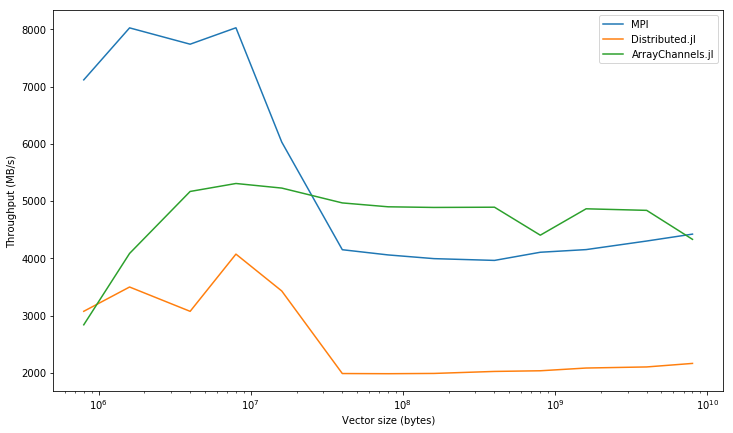
\includegraphics[width=\linewidth]{figs/pingpong.png}
  \label{fig:pingpong-results}
  \caption{Two-process Ping-Pong performance profile}
\end{figure}

In spite of \texttt{ArrayChannels.jl} being written using Julia
serialisation constructs, we still see generally improved performance
over \texttt{Distributed.jl} for larger message sizes, due to improved
cache utilisation. The largest difference in performance is attained for
40MB messages, with 150\% improvement over \texttt{Distributed.jl}. For
messages below 100kB in size, eager message passing in
\texttt{Distributed.jl} yields improved performance due to the cost of
synchronisation in the rendezvous model outweighing the benefits of
improved access locality. For message sizes up to 16MB, MPI
significantly outperforms \texttt{ArrayChannels.jl} due its highly
optimised messaging model. Interestingly, \texttt{ArrayChannels.jl}
provides up to 18\% improved performance over MPI for message sizes
ranging between 40MB and 4GB, with deteriating performance for 8GB
messages, while MPI performance continutes to increase.

\subsection{Reduce}
\label{sec:reduce-results}

In the distributed reduce kernel, each process is allocated two large
vectors so that a local reduction can be performed. For our testing
purposes, each of these vectors was 8MB in size, providing 16MB to each
process. We selected these problem sizes such that in all trials with
parallel computation, the size of program memory will exceed last-level
cache, and so highlight the effects of access locality.

The reduce kernel's performance readings depicted in figure
~\ref{fig:reduce-results} demonstrate the effect of parallelisation on
overall throughput (measured in flops per second) of the reduction
operation. In MPI, performance increases steeply with parallelisation
only for core counts above four, with only a slight increase between
three and four cores. The provision of fourteen cores in the case of MPI
provides 91\% over the sequential reading, however in both Julia
implemenations (each targeting the tree topology) provide deteriated
performance with the addition of parallelism, with fourteen cores
obtaining 84\% (with \texttt{ArrayChannels.jl}) and 46\% (with
\texttt{Distributed.jl}) of the sequential performance.\\

\begin{figure}[htb]
  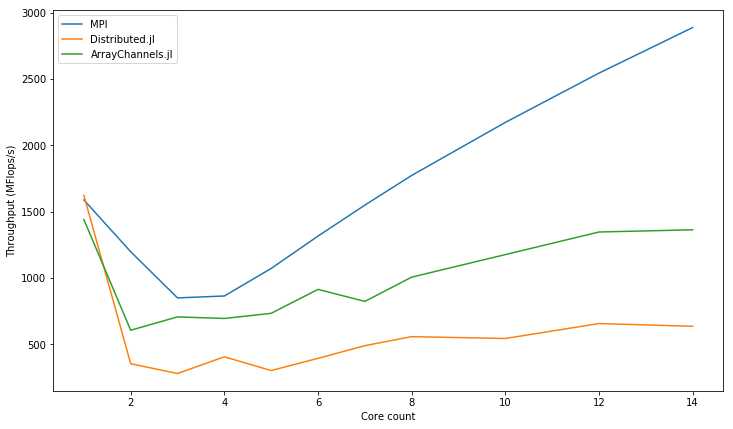
\includegraphics[width=\linewidth]{figs/reduce.png}
  \label{fig:reduce-results}
  \caption{Weak scaling on Distributed Reduction}
\end{figure}

MPI implmentations are able to target a wide variety of network
topologies in their approach to operations such as reduction, and may
even adopt different behaviour depending on the input size. By
comparison, we implement the Reduce kernel targetting exactly one
topology. In~\ref{sec:pingpong-results}, we observe that on a
shared-memory environment such as the testing environment, the MPI
implementation delivers far higher data throughput for 8MB messages than
either communication model in Julia. While the cost of communication in
Julia prohibits speedup due to parallelism on this kernel, this
performance degradation is mitigated by improved temporal locality in
\texttt{ArrayChannels.jl}.\\

\subsection{Transpose}
\label{sec:transpose-results}

In the distributed transpose kernel, all process operate on separate
portions of a large square matrix. We describe the data distribution
method in section~\ref{sec:transpose-kernel}. Each process is allocated
2MB of this matrix, however will retain a copy of their local portion
for computation.\\

In figure~\ref{fig:transpose-results}, we see that parallel performance
under Julia for the transpose kernel is greatly diminished compared to
the sequential reading and reference C-MPI code. Under
\texttt{Distributed.jl}, using parallism obtains at most 61\% of the
sequential performance, with only 50\% under \texttt{ArrayChannels.jl}.
\texttt{Distributed.jl} obtains typically higher performance than
\texttt{ArrayChannels.jl} with execution under eight cores yielding 24\%
performance improvement.\\

\begin{figure}[htb]
  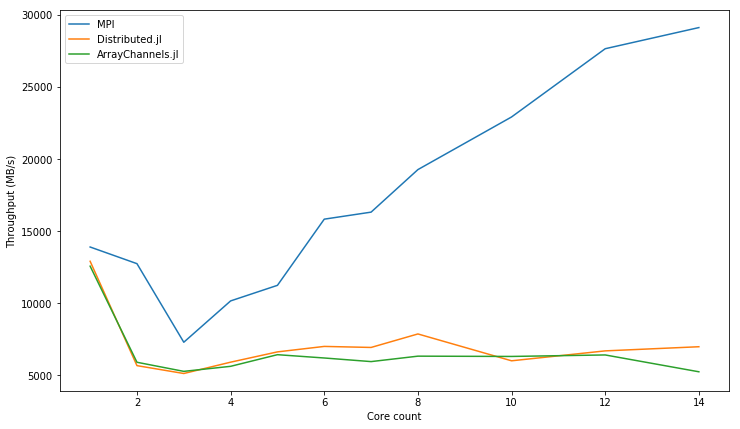
\includegraphics[width=\linewidth]{figs/transpose.png}
  \label{fig:transpose-results}
  \caption{Weak Scaling on Distributed Transpose}
\end{figure}

As with the reduce kernel, the transpose kernel's low arithmetic
intensity and large message sizes exasserbate the weaker communication
performance in Julia compared to OpenMPI. While
\texttt{ArrayChannels.jl} is able to obtain slightly improved
performance readings over \texttt{Distributed.jl} for corecounts of two
and ten (4\% and 5\% respectively), the adopted rendezvous communication
model requires an acknowledgement of the recipient's readiness to
receive prior to communicating any data. Where individual messages are
too large, and when a large number of processes must be communicated
with, this leads to occaisions where sender processes are idle when they
could instead be eagerly sending data. This leads to degraded
performance under \texttt{ArrayChannels.jl} where processes must enact
multiple communication tasks concurrently. To ensure that minimal time
is spent waiting on recipients to complete their own communication
tasks, processes may instead elect to wait on all other processes
concurrently. However, to ensure that message buffers are not
overwritten requires buffer duplication, and to facilitate this
concurrency requires increased numbers of context switches.

\subsection{Stencil}
\label{sec:stencil}

For the stencil kernel, we use the same problem sizes as with transpose,
and use a radius two `star' pointwise operator as depicted in figure
~\ref{fig:stencil-diagram}. As in transpose, processes must allocate a
copy of their local data for storing intermediate results during each
iteration, leading to an allocation of 4MB per process. In line with the
Intel PRK \footnote{Available at
  https://github.com/ParRes/Kernels/tree/master/MPI1.} implementation of
the stencil kernel, we attempt to distribute the source matrix into
roughly square regions subject to the factoring of the number of
processes.\\

All three implmentations feature typically increasing trends in
performance with the added parallelism, with improvements over
sequential readings of 11.0\(\times\), 4.19\(\times\) and 6.27\(\times\)
for MPI, \texttt{Distributed.jl} and \texttt{ArrayChannels.jl}
respectively. Between the two Julia implementations, we see up to 71\%
performance improvement for \texttt{ArrayChannels.jl} over
\texttt{Distributed.jl} with ten cores, with improved readings at each
core count we surveyed.\\

\begin{figure}[htb]
  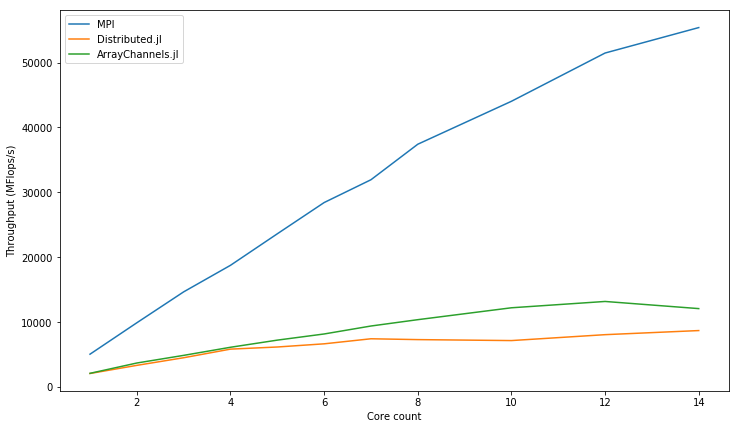
\includegraphics[width=\linewidth]{figs/stencil.png}
  \label{fig:stencil-results}
  \caption{Weak Scaling on Distributed Stencil}
\end{figure}

In the stencil kernel, messages sizes are small compared to that of
transpose or reduce, and the arithmetic intensity is high. The ghost
regions (matrix regions that must be shared between processes) have the
potential to be stored entirely in last-level cache, and as such
\texttt{ArrayChannels.jl} provides improved performance by reissuing the
same storage location when receiving the contents of these regions at
each iteration. Communication in \texttt{Distributed.jl} will instead
generate a new buffer for each incoming message, increasing memory
latency as the memory region must be fetched into processor cache prior
to use.
